\documentclass{beamer}
\usepackage[latin1]{inputenc}
\usepackage{xcolor}
\usepackage{hyperref}
\usepackage{minted}
\usepackage{graphicx}
\usepackage{tikz}
\usetikzlibrary{shapes,fit,positioning,calc}
\usepackage{bbding} % For \HandRight
\usepackage{fancyvrb} % For \UseVerb \SaveVerb

\usetheme{Madrid}
\usecolortheme{default}

% Command that embeds a hand pointing to the right in a href label
\newcommand{\hrefhand}[2]{\raisebox{-0.4ex}{\HandRight}\,\href{#1}{#2}}

\title{COMP3320 Introduction to OpenGL}
\author{Alex Biddulph}
\institute{
    The University of Newcastle, Australia
    \and
    Based on the work provided at \url{www.learnopengl.com}
}
\date{Semester 2, 2021}

\begin{document}

\begin{frame}
    \titlepage
\end{frame}

\begin{frame}[fragile]{The Open-Asset-Importer-Lib}
    \begin{itemize}
        \item Asset importer library supporting multiple 3D model formats
        \item Provides some post-processing support
        \item API provided for C/C++
        \item Languange bindings available for C\#, Java, Python, Delphi, D
        \item Can run on Android and iOS
    \end{itemize}

    \begin{examples}
        Check out \hrefhand{https://assimp.org}{\color{blue}assimp.org} for full details
    \end{examples}
\end{frame}

\begin{frame}[fragile]{Assimp Supported Formats}
    \begin{table}
        \centering
        \begin{tabular}{cccc}
            3D           & \textbf{3DS} & 3MF                  & AC              \\
            AC3D         & ACC          & AMJ                  & ASE             \\
            ASK          & B3D          & \textbf{BLEND}       & BVH             \\
            CMS          & COB          & \textbf{DAE/Collada} & DXF             \\
            ENFF         & FBX          & glTF 1.0 + GLB       & glTF 2.0        \\
            HMB          & IFC-STEP     & IRR / IRRMESH        & LWO             \\
            LWS          & LXO          & MD2                  & MD3             \\
            MD5          & MDC          & MDL                  & MESH / MESH.XML \\
            MOT          & MS3D         & NDO                  & NFF             \\
            \textbf{OBJ} & OFF          & OGEX                 & PLY             \\
            PMX          & PRJ          & Q3O                  & Q3S             \\
            RAW          & SCN          & SIB                  & SMD             \\
            STP          & \textbf{STL} & TER                  & UC              \\
            VTA          & X            & X3D                  & XGL             \\
                         &              & ZGL                  &
        \end{tabular}
    \end{table}
\end{frame}

\begin{frame}[fragile]{Assimp Post Processing Support}
    \begin{itemize}
        \item Normal generation
        \item Tangent generation
        \item Triangulation
        \item Removal of degenerate primitives
        \item Removal of duplicate vertices
        \item Index generation
        \item Lots more
    \end{itemize}
\end{frame}

\begin{frame}[fragile]{Assimp Model Structure}
    \begin{figure}
        \centering
        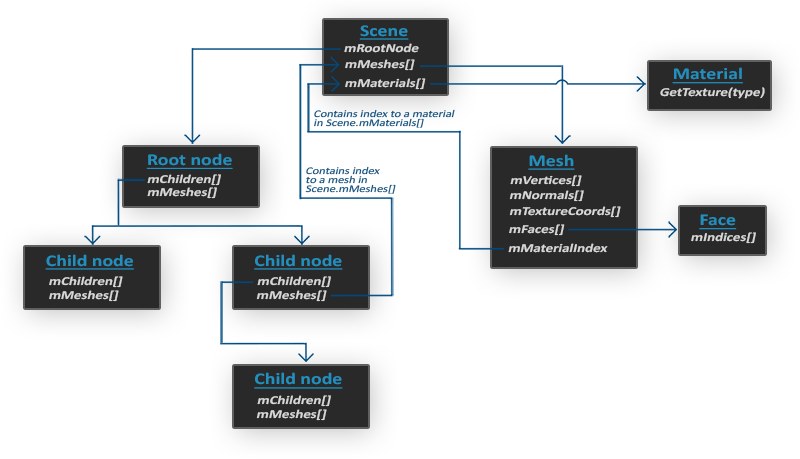
\includegraphics[width=0.95\linewidth]{images/assimp_structure.png}
        \caption{\footnotesize{Image sourced from \url{learnopengl.com/Model-Loading/Assimp}}}
    \end{figure}
\end{frame}

\begin{frame}[fragile]{Assimp Model Structure}
    \SaveVerb{scene}|Scene|
    \SaveVerb{root}|Root Node|
    \SaveVerb{mesh}|Mesh|
    \SaveVerb{face}|Face|
    \SaveVerb{material}|Material|
    \begin{itemize}
        \item \hrefhand{https://assimp-docs.readthedocs.io/en/latest/API/API-Documentation.html\#_CPPv47aiScene}{\color{blue}\UseVerb{scene}} is the root node of the imported model
        \item {\color{blue}\UseVerb{scene}} contains all meshes and materials as well as a link to root node of the meshes
        \item {\color{blue}\UseVerb{root}} starts a tree structure that contains links to meshes and child nodes
        \item Each \hrefhand{https://assimp-docs.readthedocs.io/en/latest/API/API-Documentation.html\#_CPPv46aiMesh}{\color{blue}\UseVerb{mesh}} contains vertices, normals, texture coordinates, faces, and a link to
              materials (textures)
        \item Only vertices and faces is guaranteed to be in a {\color{blue}\UseVerb{mesh}}, the rest are only there if
              they were in the model or you asked Assimp to calculate them for you
        \item Each \hrefhand{https://assimp-docs.readthedocs.io/en/latest/API/API-Documentation.html\#_CPPv46aiFace}{\color{blue}\UseVerb{face}} contains indices
        \item Each \hrefhand{https://assimp-docs.readthedocs.io/en/latest/API/API-Documentation.html\#_CPPv410aiMaterial}{\color{blue}\UseVerb{material}} contains information about a texture
    \end{itemize}
\end{frame}

\begin{frame}[fragile]{Assimp and OpenGL}
    \SaveVerb{scene}|Scene|
    \SaveVerb{vertex}|Vertex|
    \SaveVerb{mesh}|Mesh|
    \SaveVerb{render}|model.render()|
    \begin{itemize}
        \item Not geared at OpenGL
        \item Best to restructure the {\color{blue}\UseVerb{scene}} data to make it easier to work with OpenGL
              \begin{itemize}
                  \item Create our own {\color{blue}\UseVerb{vertex}} class which encapsulates position, normal, and texture
                        coordinates
                  \item Create our own {\color{blue}\UseVerb{mesh}} class which encapsulates VAOs, VBOs, EBOs,
                        {\color{blue}\UseVerb{vertex}} data, and textures
                  \item The {\color{blue}\UseVerb{mesh}} class will also bind its own textures and render its own indices/vertices
                  \item The program's main render loop can now be reduced to calling {\color{blue}\UseVerb{render}} for
                        each loaded model and setting up uniforms for lighting
              \end{itemize}
    \end{itemize}
\end{frame}

\begin{frame}[fragile]{OpenAL}
    \begin{itemize}
        \item Software interface for audio hardware
        \item Meant to resemble the OpenGL API
        \item A means to generate audio in a simulated 3D space
        \item OpenAL includes both the core API as well as OS bindings (unlike OpenGL)
        \item Can handle sound source directivity, distance-related attenuation, Doppler effects, and environmental
              effects
              \begin{itemize}
                  \item Reflection,
                  \item Obstruction,
                  \item Transmission, and
                  \item Reverberation
              \end{itemize}
    \end{itemize}
\end{frame}

\begin{frame}[fragile]{OpenAL Structure}
    \begin{figure}
        \centering
        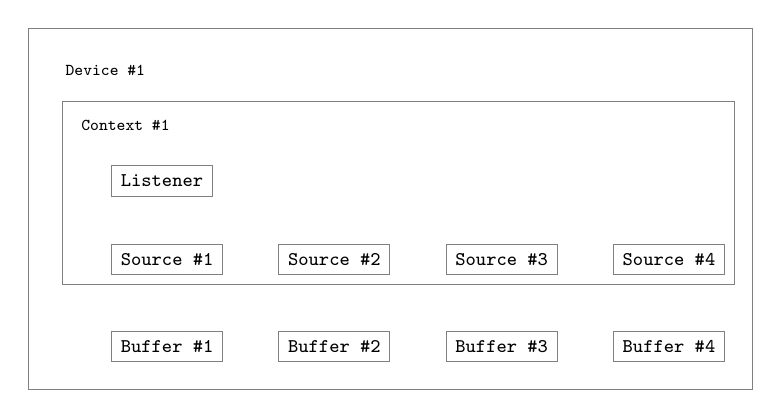
\begin{tikzpicture}[
                node distance=7mm,
                title/.style={font=\fontsize{6}{6}\color{black}\ttfamily},
                contexttag/.style={rectangle, draw=black!50, font=\scriptsize\ttfamily, anchor=west},
                devicetag/.style={rectangle, draw=black!50, font=\scriptsize\ttfamily}
            ]
            \node (device) [title] {Device \#1};

            \node (context) [below=of device.west, title, anchor=west, xshift=2mm] {Context \#1};

            \node (listener) [below=of context.west, contexttag, xshift=5mm] {Listener};
            \node (source1) [below=of context.west, contexttag, xshift=5mm, yshift=-1.0cm] {Source \#1};
            \node (source2) [right=of source1.east, contexttag] {Source \#2};
            \node (source3) [right=of source2.east, contexttag] {Source \#3};
            \node (source4) [right=of source3.east, contexttag] {Source \#4};

            \node [draw=black!50, fit={(context) (listener) (source1) (source2) (source3) (source4)}] {};

            \node (buffer1) [below=of source1.south, devicetag] {Buffer \#1};
            \node (buffer2) [right=of buffer1.east, devicetag] {Buffer \#2};
            \node (buffer3) [right=of buffer2.east, devicetag] {Buffer \#3};
            \node (buffer4) [right=of buffer3.east, devicetag] {Buffer \#4};

            \node [inner sep=10pt, draw=black!50, fit={(device) (context) (buffer1) (buffer2) (buffer3) (buffer4)}] {};
        \end{tikzpicture}
        \caption{\footnotesize{Image recreated from \hrefhand{https://www.openal.org/documentation/OpenAL_Programmers_Guide.pdf}{\color{blue}OpenAL Programmers Guide, Page 8}}}
    \end{figure}
\end{frame}

\begin{frame}[fragile]{OpenAL Structure}
    \SaveVerb{buffer}|Buffer|
    \SaveVerb{source}|Source|
    \SaveVerb{listener}|Listener|
    \SaveVerb{libsndfile}|libsndfile|
    \begin{itemize}
        \item {\color{blue}\UseVerb{buffer}}s are filled with audio data
              \begin{itemize}
                  \item Need to use an external library for this, similar to OpenGL and textures
                  \item \hrefhand{http://libsndfile.github.io/libsndfile/}{\color{blue}\UseVerb{libsndfile}} is one option for this
                  \item \hrefhand{http://libsndfile.github.io/libsndfile/formats.html}{\color{blue}Supported formats and encodings} can be seen here
              \end{itemize}
        \item A {\color{blue}\UseVerb{buffer}} is then attached to a {\color{blue}\UseVerb{source}}
        \item There can be multiple {\color{blue}\UseVerb{source}}s per context
        \item A {\color{blue}\UseVerb{source}} has a position and an orientation (and other properties)
        \item The position and orientation of a {\color{blue}\UseVerb{source}} relative to the {\color{blue}
                      \UseVerb{listener}} dictates how the {\color{blue}\UseVerb{source}} is heard
        \item There can only be $1$ {\color{blue}\UseVerb{listener}} per context
        \item Update the positions, orientations, and velocities of the {\color{blue}\UseVerb{listener}} and
                  {\color{blue}\UseVerb{source}}s dynamically to get convincing 3D audio effects
    \end{itemize}
\end{frame}

\begin{frame}[fragile]{OpenAL Properties}
    \SaveVerb{source}|Source|
    \SaveVerb{listener}|Listener|
    \SaveVerb{position}|position|
    \SaveVerb{up}|up|
    \begin{itemize}
        \item {\color{blue}\UseVerb{listener}} properties
              \begin{itemize}
                  \item Gain
                  \item Position
                  \item Velocity
                  \item Orientation ({\color{blue}\UseVerb{position}} and {\color{blue}\UseVerb{up}})
              \end{itemize}
        \item {\color{blue}\UseVerb{source}} properties
              \begin{itemize}
                  \item Pitch
                  \item Min gain, Gain, Max gain
                  \item Max distance, Reference distance
                  \item Rolloff factor
                  \item Position, velocity, direction
                  \item Source relative
                  \item Looping
                  \item .... many more
              \end{itemize}
    \end{itemize}
\end{frame}

\begin{frame}[fragile]{OpenAL Workflow}
    \begin{enumerate}
        \item Determine which playback device you want to use via enumeration and open it
              \begin{itemize}
                  \item If there is only one playback device on your system you can use the default device
              \end{itemize}
        \item Create and open a context on the device
        \item Set up initial listener properties
        \item For each source
              \begin{enumerate}
                  \item Create source and set properties
                  \item Load in audio data to a raw PCM format and transfer to OpenAL buffer
                  \item Associate buffer with OpenAL source
              \end{enumerate}
        \item Play sources when deemed appropriate
              \begin{itemize}
                  \item OpenAL will play sources asynchronously
              \end{itemize}
    \end{enumerate}
\end{frame}

\begin{frame}[fragile]{More Information}
    \begin{examples}
        See \hrefhand{https://www.openal.org/documentation/OpenAL_Programmers_Guide.pdf}{\color{blue}OpenAL Programmers Guide} for more details on using OpenAL
    \end{examples}

    \begin{examples}
        See \hrefhand{https://ffainelli.github.io/openal-example/}{\color{blue}OpenAL short example} for brief tutorial
    \end{examples}
\end{frame}

\end{document}
